% SPDX-FileCopyrightText: Copyright (c) 2019-2025 CQFN.org
% SPDX-License-Identifier: MIT

\subsection{The Idea}

The main purpose of Aibolit is to help developers identify  patterns in their
code that may cause maintainability issues. From the user perspective, it works
by outputting a list of patterns recommended to remove, given a Java class. The
Aibolit engine is comprised of two parts: an ML regression model and a
recommendation algorithm. The regression model  predicts maintainability of any
Java class. The recommendation algorithm uses the regression model to decide
which pattern is better to avoid by considering different various modifications
of the input Java class.

\begin{figure}[t]
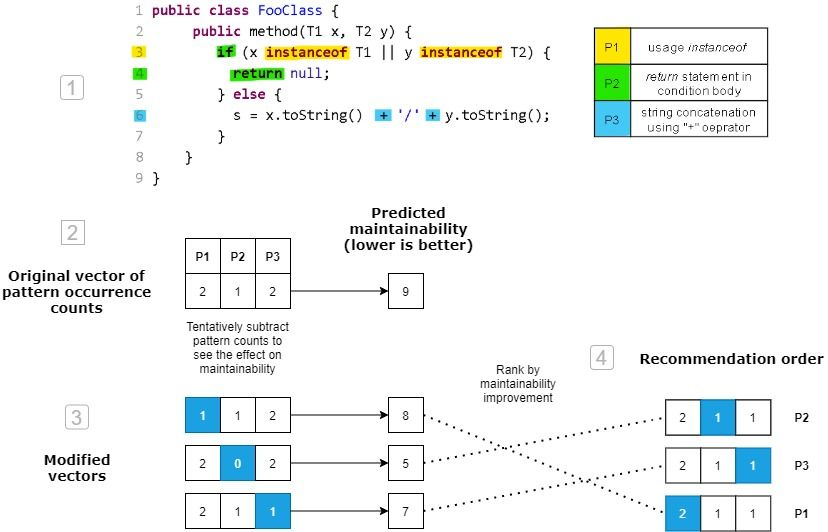
\includegraphics[width=13cm]{how_it_works_diagram_5.jpg}
\centering
\vspace{1 cm}
\caption{How Aibolit works: (1) Inspect the source code for patterns.
(2) Count the pattern occurrences and put them in a vector representation.
Compute the maintainability metric value for the vector.
(3) Consider changes to the vector representation by subtracting pattern counts.
Predict the corresponding maintainbility metric score.
(4) Rank all the alternative vectors wrt to how much they improve the original
maintainability score. Recommend changes that gave the most improvement.}
\label{fig:aibolit_graphic}
\end{figure}

Figure~\ref{fig:aibolit_graphic} represents the Aibolit recommendation proceduce on high level.
In the remaining subsections we provide a more detailed
description of each of Aibolit's components.

\subsection{Patterns \& Quality metrics}
\label{sec:aibolit_patterns_metrics}

\subsubsection*{Patterns}

As discussed above (Section~\ref{sec:related}),
software engineering researchers and practitioners often associate
good and bad code design with specific patterns. We follow this tradition and
build a predictive system to reason about observed patterns in code in terms of their effect on quality.
In the current release of Aibolit, the model is built on top of 34
commonly used manually designed patterns as input features. See Appendix
for the complete list and detailed descriptions. Note that users of Aibolit
can arbitrarily extend the model by implementing and integrating their patterns
of choice.

\subsubsection*{Metrics}

The ultimate goal behind Aibolit's approach is to
learn to identify maintainability-affecting patterns in code and recommend them
to the user. However, as discussed above, maintainability quantification is
still an open problem, and most of the metrics proposed so far typically
describe only a narrow aspect of software maintainability. We recognize it as
the major challenge of our approach and plan to research this problem in the
future.

In the current release of Aibolit, we use Cognitive Complexity \citep{10.1145/3194164.3194186} as
the maintainability metric. We refer to it as the maintainability metric or just
metric in the remainder of the text.

\subsection{Maintainability prediction model}

\label{sec:maint_pred_model}

\subsubsection*{Dataset}

\label{sec:dataset}

To train our prediction model, we mined training data
from Github open source repositories. We chose repositories written in Java
as the main language. We filtered out all non-Java files and all software
testing files. To make sure our data is
representative of good software engineering standards, we only extracted
repositories with at least 100 starts and at least six collaborators.

Aibolit is currently designed to do predictions and recommendations at class
level. For simplicity, we only consider files that contain exactly one
non-abstract Java class.
%We chose this level of granularity because it is intuitive and because we
%wanted to narrow down our scope for the first stage of development. Thus one
%datapoint in our dataset is one Java class.
We filtered out classes with fewer than 50 and more than 300 lines of code.
The resulting filtered dataset consists of 124 repositories and
29,065 classes. Before filtering, we split the dataset into a test and train sets randomy by files with
approximately 0.7:0.3 ratio. The filtered train set contains 20,049 classes,
the filtered test contains 9,016.
%More detailed statistics can be found in Table~\todo. -- keep this for research paper
The complete list of mined repositories and the train/test split is provided in Aibolit
project folder.
%(\todo link to file with repository URLs).

\subsubsection*{Feature and target preprocessing}

Each Java class gets
associated with a vector of numerical features. We use scaled pattern counts as
features. For each pattern from the fixed set
(see Appendix), we count its occurrences in the
class and divide it by the number of non-commented lines in the class (NCSS).
The target value for each datapoint is the maintainability metric value for the
class (Section~\ref{sec:aibolit_patterns_metrics}), also divided by the NCSS.
%(\ref{eq:feat_vector}) and (\ref{eq:targ_val}) summarize feature and target
%value computation (where $f_p^C$ is the feature value for pattern $p$ and code
%$C$, $t^C$ is the target value for code $C$	).
Table~\ref{tab:features_example}
gives an illustration of how a dataset looks like after the this procedure.


%\vspace{0.2in}
%
%\begin{minipage}{.4\linewidth} \begin{equation} \label{eq:feat_vector} f_p^C =
%\frac{\textit{count}(p, C)}{\textit{NCSS}(C)}\end{equation} \end{minipage}%
%\begin{minipage}{.55\linewidth} \begin{equation} \label{eq:targ_val} t^C =
%\frac{\textit{Metric}(C)}{\textit{NCSS}(C)} \end{equation} \end{minipage}
%
%\vspace{0.2in}


We apply NCSS scaling because we observed that our maintainability metric
(Cognitive Complexity) is highly correlated with code size. The scaling
stimulates the model to find more implicit  dependencies between patterns and
complexity.

\begin{table}[H] \begin{center} \begin{tabular}{|r|rrrr|r|} \hline \textbf{class
id} & \textbf{P16} & \textbf{P11} &  \textbf{P13} & \dots & \textbf{CogC}
(target metric) \\ \hline \hline class 1 & 0.008695 & 0.         & 0.026086 &
\dots&  0.417391 \\ class 2 & 0.              & 0.05      & 0.116667 & \dots&
0.466667 \\  class 3 & 0.009909 & 0.         & 0.009909 & \dots & 0.732673 \\
\hline \end{tabular} \end{center} \caption{Example of a training dataset with
preprocessed feature values. \textbf{P16}: {\em Return null}, \textbf{P11}: {\em
Multiple Try},  \textbf{P13}: {\em Null checks}).} \label{tab:features_example}
\end{table}



\subsubsection*{Training}
We train a gradient boosting regression model \citep{Friedman2001GreedyFA}.
We use the implementation of CatBoost \citep{Dorogush2018CatBoostGB} with the RMSE loss function.
For hyperparameter selection, we do a 3-fold crossvalidation.


\subsection{Recommendation algorithm}
\label{sec:recommendation_algorithm}
Our recommendation algorithm ranks
patterns observed in the user's source class according to their individual
impact on the code's maintainability metric value. It then outputs a pattern
with the \textit{most negative impact} as a recommendation to the user to remove
it from their code.

For each pattern $p$ we compute the \textbf{impact factor} $I_{\textit{neg}}(p, C)$
on code $C$, which is intended to capture the \textit{negative
influence} of $p$ on $C$. It is the difference between the quality metric value
of the original code $C$ and the version of $C$ where the count of $p$ has been
decreased (Eq.~\ref{eq:impact_factor}):

\begin{equation} \label{eq:impact_factor} I_{\textit{neg}}(p_i, C) = M(F(C)) -
M(F_{p_{i} - 1}(C)), \end{equation}

where $M$ is a quality metric, $F(C)$ is the feature vector $\langle f^C_{p_1},
..., f^C_{p_n} \rangle$, $F_{p_{i} - 1}(C)$ is the feature vector with the count
of $p_i$ decreased by $1$.%: $\langle f^C_{p_1}, ..., f^C_{p_i - 1}, ...,
%f^C_{p_n} \rangle$. With $f^C_{p_i - 1}$ computed as:\footnote{We chose to
%subtract 1, but in principle it is a hyperparameter of our model and we plan to
%experiment with other values.}

%\begin{equation} \label{eq:feature_count_min_1} f_{p_i - 1}^C =
%\frac{\textit{count}(p_i, C) - 1}{\textit{NCSS}(C)} \end{equation}

Under the ``lower metric is better'' convention (i.e., lower value of quality metric
means better quality), lower values of $I_{\textit{neg}}$ correspond to patterns
that contribute more to the deterioration of the code's quality. We rank pattern
according to their $I_{\textit{neg}}$ and output patterns with lowest values as
recommendations.

Note that at the moment of recommendation we do not observe code with a
decreased pattern count, so we cannot compute the maintainability metric
directly. This is why we resort to a predictive maintainability model
(Section~\ref{sec:maint_pred_model}), which helps estimate maintainability of a
hypothetical code.



\textbf{Algorithm}~\ref{fig:recsys_alg} summarizes how we do recommendations.
For each pattern from the set of patterns used at training, we
precompute feature values and compute the metric value of the source code
(lines~\ref{line:init_F}-\ref{line:compute_m_source}). Then we compute the
impact factor $I_p$ of each pattern $p$ on the source code maintainability
(lines~\ref{line:init_I}-\ref{line:impact}). Under ``lower is better''
convention of maintainability metric, low values of $I_p$ indicate that removal
of $p$ lead to improvement of the metric score. We collect the $K$ most
negatively impacting patterns and output them as recommendations.  Thus, we
 pick patterns $p$ for which $I_p$ are the highest
(lines~\ref{line:topK}-\ref{line:return}).

\begin{algorithm}[t]
\caption{Aibolit recommendation algorithm}
\hspace{\algorithmicindent}
\textbf{Input:}  $\mathsf{M}$: pretrained
maintainability model); $C$: class source code; \\
\hspace{\algorithmicindent} $P$: array of patterns used for training $\mathsf{M}$\\

\begin{algorithmic}[1]
\State $F = [ ]$ \label{line:init_F}
\For{\texttt{i = 1, $|P|$}}
\State $F[i] =\frac{\textit{count}(P[i], C)}{\textit{NCSS}(C)}$% (Eq.~\ref{eq:feat_vector})
\EndFor \State $M_{\textit{observed}} = \mathsf{M}(F)$ \label{line:compute_m_source}
\State $I = [ ]$ \label{line:init_I}
\For{\texttt{i = 1, $|P|$}}

\State $F^{\prime} = F$
\State $F^{\prime}[i] = F[i] - \frac{1}{\textit{NCSS}(C)}$ \label{line:f_prime} %(Eq.~\ref{eq:feature_count_min_1})
\State $I[i] = M_{\textit{observed}} - \mathsf{M}(F^{\prime})$ \label{line:impact} % (Eq.~\ref{eq:impact_factor})
\EndFor
\State $I_{\textit{worst}} = \texttt{topK}_{i \in [1,...,|P|]} (-I[i])$ \label{line:topK}
\State \textbf{return} $\{P[i]~|~i \in I_{\textit{worst}}\}$ \label{line:return}

\end{algorithmic}
\centering
\label{fig:recsys_alg}
\end{algorithm}


% \subsection{How to customize Aibolit} label{sec:customizing_aibolit}

% By design, Aibolit is easily adjustable and extendable. It gives an end user
% the opportunity to adapt the tool to their own requirements and preferences.
% Aibolit's core mechanism is ML-driven, therefore, as the user adds new
% patterns to the system, there is no need to manually specify how the pattern
% should be used by the tool. The interactions between patterns are discovered
% automatically by the learning algorithm.

% In order to modify the set of patterns, the user should provide an
% implementation of a pattern extractor for source code file and modify the
% configuration file (\verb|aibolit/config.py|) accordingly. See full
% instructions in \todo (shouldn't we add them in README?)

% In order to change the quality metric for training the prediction model, ???
% \todo.
